% To build everything run
%	latexmk -xelatex
% To clean temporary files run
%	latexmk -c
\documentclass[12pt]{scrreprt}

% German locale *************************
\usepackage[T1]{fontenc}
\usepackage[ngerman]{babel}
%****************************************

% Use Verbose citation ******************
%\usepackage[natbibapa]{apacite}
\usepackage{csquotes}
\usepackage{url}
\usepackage[
	backend		= biber,
	style			= verbose,
	autocite	= footnote
	]{biblatex}
	\bibliography{ling-relativ-prinzip}
%****************************************

% Add images ************
\usepackage{graphicx}
%****************************************

% Configure captions ********************
\usepackage[
	format			= hang,
	labelfont		= bf,
	font				= bf,
	figurename	= Abb.,
	tablename		= Tab.
	]{caption}
%****************************************

% Blind text*****************************
\usepackage{lipsum}
%****************************************

% Define itemize bullets ****************
\renewcommand{\labelitemi}{$\bullet$}
\renewcommand{\labelitemii}{$\circ$}
\renewcommand{\labelitemiii}{$\bullet$}
\renewcommand{\labelitemiv}{$\circ$}
%****************************************

% Define enumerate numbers ****************
\renewcommand{\labelenumii}{\arabic{enumi}.\arabic{enumii}}
\renewcommand{\labelenumiii}{\arabic{enumi}.\arabic{enumii}.\arabic{enumiii}.}
\renewcommand{\labelenumiv}{\arabic{enumi}.\arabic{enumii}.\arabic{enumiii}.\arabic{enumiv}.}
%****************************************

% Configure fonts ***********************
% Comment out when fonts are not
% found or use different fonts
%\usepackage{lmodern}
\usepackage{fontspec}
	\setmainfont{TeX Gyre Pagella}
	\setsansfont{TeX Gyre Heros}
%****************************************

% Define layout *************************
\usepackage{setspace}
	\setstretch{1.41}
\usepackage[
	a4paper,
	left		= 2.5cm,
	right		= 3cm,
	top			= 2cm,
	bottom	= 2cm,
	%includeheadfoot,
	%showframe
	]{geometry}
%****************************************

%****************************************
\usepackage{scrlayer-scrpage}
\usepackage[bottom]{footmisc}
	\clearpairofpagestyles

	\setkomafont{pageheadfoot}{\rmfamily}
	%\setkomafont{pagehead}{\bfseries}
	\setkomafont{pagination}{}

	\KOMAoptions{
	   headsepline	= true,
	   footsepline	= false,
	   %plainfootsepline	= true,
	}

	\automark[chapter]{chapter}

	\ihead{\headmark}
	\ohead{\pagemark}
%****************************************

% Make titlepage ************************
\usepackage{titlepage}
	\ititle{Das linguistische Relativitätsprinzip}
	\isubtitle{Sapir-Whorf-Hypothese} % Optional
	\iauthor{Jasper Gude}
	\idate{\today}
	\irefnr{}
	\iaddress{Hockenheim} % Only for ireports!
%****************************************

\begin{document}

\makeititle
%***************
\begin{center}
	\sffamily\bfseries{Eigenständigkeitserklärung}
\end{center}
Ich versichere, dass ich diese Ausarbeitung selbständig verfasst, alle aus
anderen Werken wörtlich oder sinngemäß entnommenen Stellen unter Angabe der
Quelle als Entlehnung kenntlich gemacht und andere als die angegebenen
Hilfsmittel nicht benutzt habe.

Oftersheim, \today, Unterschrift
%***************
\tableofcontents
%***************
\listoffigures
%***************
\listoftables
%***************
\chapter{Vorwort}
	\label{chap:vorwort}
\textquote{
\enquote{Wie hängen Sprache, Denken und Wirklichkeit
zusammen?} – Das \enquote{linguistische Relativitätsprinzip} von Benjamin Le
Whorf
\smallskip\newline
Inwiefern ist Sprache ein Medium der Erkenntnis?
Was ist dahingehend die Ansicht der aktuellen Neurowissenschaft?}
\bigskip\newline
Als GFS-Thema hat mich diese Fragestellung sehr angeprochen.
Die Deutschthemen der Klassenstufen davor erschienen mir oft entweder sehr
trocken, oder sehr willkürlich.

Bei diesem Thema gefiel mir direkt der wissenschaftliche Ansatz, der in die
psychologische und neurologische Richtung geht, auch wenn ich zugeben muss, dass
mich diese Bereiche der Wissenschaft zwar interessieren, ich mich damit aber nie
besonders tiefreichend beschäftigt habe.

Ein nettes Nebenprodukt dieser GFS wird also die Erweiterung meines
wissenschaftlichen Horizonts sein.

\chapter{Einleitung}
\label{chap:einleitung}

\chapter{Benjamin Lee Whorf}
\label{chap:bjwhorf}
Benjamin Lee Whorf wird am 24. April 1897 in Winthrop, Massachussetts geboren
und starb früh im Alter von 44 Jahren in Wethersfield, Connecticut.
\begin{figure}[!htb]
	\centering
	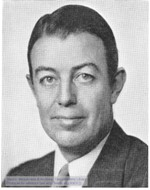
\includegraphics[width=0.25\textwidth]{whorf}
	\caption[Benjamin Lee Whorf {\autocite{image:B_L_Whorf}}]{Benjamin Lee Whorf\footnotemark}
	\label{fig:whorf}
\end{figure}
\footcitetext{image:B_L_Whorf}\\
Zu seinen populärsten Arbeiten als Amateurlinguist zählen vor allem die Arbeiten,
zu den amerikanischen Eingeborenensprachen, wie etwa die der Hopi, als auch die
These der \enquote{sprachlichen Relativität}, um die es in dieser Facharbeit
gehen soll.

	\section{Leben und Werk}
	\label{sec:lebenuwerk}
	Whorf schließt 1928 das Chemietechnik-Studium am Massachusetts Institute of
	Technology (MIT) ab und fängt bei einer Versicherungsgesellschaft als
	Brandverhütungs-Inspektor an, zu arbeiten. Bei diesem Unternehmen wird er
	zeitlebens bleiben und Karriere machen.

	Sein Interesse an der Wissenschaft lindert dies jedoch nicht. Whorf lernt
	Hebräisch und forscht im Bereich der aztekischen Nahua-Sprachen und der
	Maya-Sprachen. Seine Erkenntnisse kommen jedoch zu früh und treffen auf wenig
	Begeisterung.
		\subsection{Einflüsse}
		\label{sec:einfluesse}
		Zu Benjamin Whorfs größten Einflüssen zählt Edward Sapir. Als dieser zum
		\textit{Sterling Professor für Linguistik und Anthropologie} an der
		Universität Yale ernannt wird, fängt Whorf sofort an, bei ihm amerikanische
		indianische Linuistik zu studieren.

		Dabei macht Sapir ihn auf die Sprache der Hopi aufmerksam, die er durch
		Informanten in New York lernt. In der Zeit danach entstehen mehrere Arbeiten,
		die zum Teil erst nach seinem Tod veröffentlicht werden.

		Den Denkanstoß in Richtung der Entwicklung seiner Hypothese, die später als
		Sapir-Whorf-Hypothese bekannt wird, gibt ihm seine Arbeit für die
		Versicherungsgesellschaft.

		Bei einem der Fälle ging es um einen Unfall, bei dem eine Flasche mit der
		Aufschrift \enquote{highly inflammable} neben einer Heizung Abgestellt wurde
		der Arbeiter, dessen Muttersprache nicht Englisch war, ging davon aus, dass
		\enquote{inflammable} unbrennbar hieße, da \enquote{flammable} brennbar
		heißt. Da die Vorsilbe \enquote{in-} nicht immer das Gegenteil ausdrückt,
		kam es zum Entzünden der Flasche.\autocite{wiki:Benjamin_Lee_Whorf}

\chapter{Sapir-Whorf-Hypothese}
\label{chap:sphypothese}
	\section{Interpretationen post mortem}
	\label{sec:interpretpm}
		\subsection{Das Prinzip der linguistischen Relativität}
		\label{sec:lingrelativ}
		\begin{figure}[!htb]
			\centering
			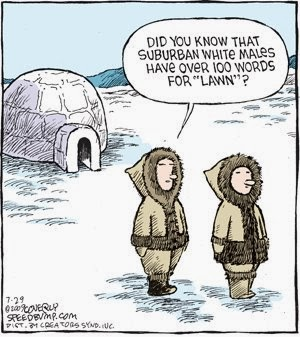
\includegraphics[width=0.5\textwidth]{inuitcartoon}
			\caption[Kritik an den Belegen Whorfs {\autocite{cartoon:Inuit}}]{Kritik an den Belegen Whorfs\footnotemark}
			\label{fig:nutzlos}
		\end{figure}
		\footcitetext{cartoon:Inuit}

		\subsection{Das Prinzip des linguistischen Determinismus}
		\label{sec:lingdetermin}
	\section{Aktualität der Hypothese}
	\label{sec:aktualität}
		\subsection{Neue empirische Forschung}
		\label{sec:empforschung}
		\subsection{Das grammatische Geschlecht}
		\label{sec:gramgeschlecht}

\chapter{Lehnwörter}
\label{chap:lehnwörter}

\begin{table}[!htb]
	\centering
	\caption[Nutzlose Tabelle {\autocite{a}}]{Nutzlose Tabelle\footnotemark}
	\begin{tabular}{ |c|c|c| }
		\hline
		cell1 & cell2 & cell3 \\
		\hline
		cell4 & cell5 & cell6 \\
		cell7 & cell8 & cell9 \\
		\hline
	\end{tabular}
	\label{tab:nutzlos}
\end{table}
\footcitetext{a}

\begin{figure}[!htb]
	\centering
	\includegraphics[width=0.5\textwidth]{example-image-a}
	\caption[Nutzlose Abbildung {\autocite{c}}]{Nutzlose Abbildung\footnotemark}
	\label{fig:nutzlos}
\end{figure}
\footcitetext{c}

\subsubsection{Unterunterabschnittüberschrift}
	\label{sec:unterunterabschnitt}

\begin{itemize}
	\item Lorem ipsum dolor sit amet
	\item Lorem ipsum dolor sit amet
	\begin{itemize}
		\item Lorem ipsum dolor sit amet
		\item Lorem ipsum dolor sit amet
		\item Lorem ipsum dolor sit amet
		\begin{itemize}
			\item Lorem ipsum dolor sit amet
			\item Lorem ipsum dolor sit amet
			\item Lorem ipsum dolor sit amet
		\end{itemize}
	\end{itemize}
	\item Lorem ipsum dolor sit amet
\end{itemize}

\begin{enumerate}
	\item Lorem ipsum dolor sit amet
	\item Lorem ipsum dolor sit amet
	\begin{enumerate}
		\item Lorem ipsum dolor sit amet
		\item Lorem ipsum dolor sit amet
		\item Lorem ipsum dolor sit amet
		\begin{enumerate}
			\item Lorem ipsum dolor sit amet
			\item Lorem ipsum dolor sit amet
			\item Lorem ipsum dolor sit amet
		\end{enumerate}
	\end{enumerate}
	\item Lorem ipsum dolor sit amet
\end{enumerate}

\printbibliography

\end{document}
